\section{基于大模型的智能问答系统}

\subsection{系统目标}

本项目在网站中集成了一个基于本地知识库的智能问答模块。用户可以直接输入自然语言问题，例如“LINE-1 相关疾病有哪些”“LINE-1 相关功能是什么”“L1HS 和 LINE-1 是什么关系”或“哪些文献支持 LINE-1 与阿尔茨海默病相关”。系统需要结合本地 Neo4j 图数据库中的知识，给出结构化且带有参考文献的回答，而不是脱离知识库进行自由生成。

与普通聊天系统不同，本项目的问答模块强调“基于本地知识库回答”和“附带证据来源”两点。一方面，系统回答的核心内容应来自已导入的转座元件知识图谱；另一方面，回答中需要尽可能返回 PMID 或文献标题，以满足课程项目对于知识溯源的要求。

\subsection{RAG 架构设计}

本系统的智能问答模块采用检索增强生成（Retrieval-Augmented Generation, RAG）架构。其核心思想是：先从本地图数据库中检索与用户问题相关的结构化知识，再将这些检索结果作为上下文提供给大模型，由模型生成通顺、客观、学术化的自然语言回答。

考虑到完全自由的 Text2Cypher 在课程项目场景下容易产生不可控的错误，本项目采用了“模板优先、Text2Cypher 兜底”的策略。对于常见且结构清晰的问题，优先匹配模板化查询；仅在模板未命中时，才进入受限的 Text2Cypher 生成流程。这种设计在保持灵活性的同时，提高了系统稳定性和可演示性。

\begin{figure}[H]
  \centering
  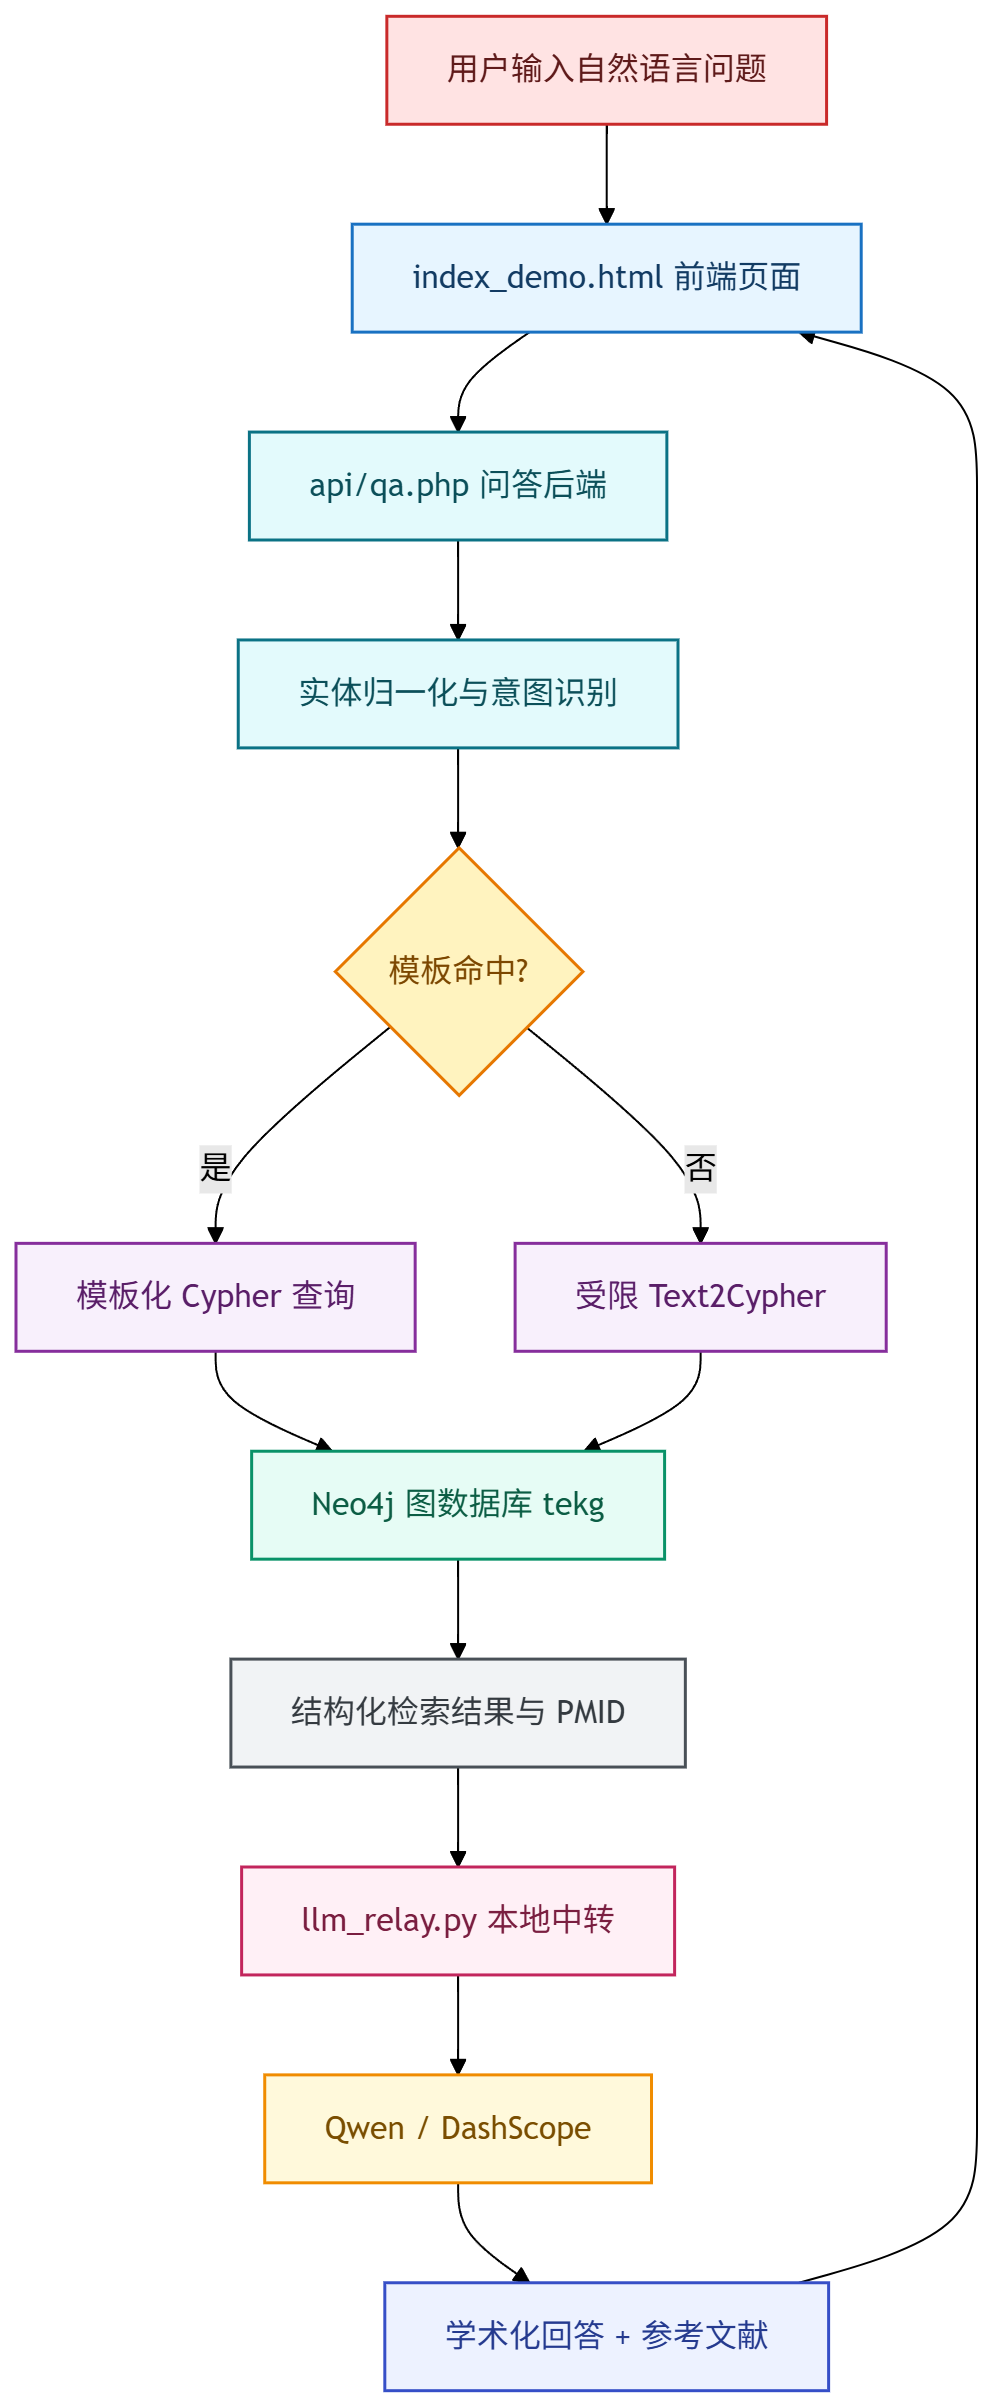
\includegraphics[width=0.88\linewidth]{figures/fig_rag_architecture.png}
  \caption{基于 Neo4j 检索与 Qwen 生成的 RAG 问答架构}
  \label{fig:rag}
\end{figure}

\subsection{Prompt 设计思路}

Prompt 设计的核心目标是约束模型只基于本地检索结果作答，并以较为严谨的学术语言组织回答。具体而言，本项目在提示词设计中遵循以下原则：

\begin{itemize}[leftmargin=2em]
  \item 明确要求模型优先依据 Neo4j 检索结果回答，而不是自由发挥；
  \item 要求回答采用固定结构，如“结论”“关键点”“参考文献”三段式；
  \item 要求在可提供文献时尽量附带 PMID 或文献标题；
  \item 若知识库中缺乏充分证据，则明确说明“本地知识库暂无充分证据”，避免模型编造关系；
  \item 对输出语言进行约束，使其尽量保持客观、严谨和适合作业展示的风格。
\end{itemize}

此外，系统还对一些常见术语进行了后处理规范化，例如疾病名称中英混杂、实体名称别名不统一等问题，以提升最终回答的可读性和一致性。

\subsection{问答流程实现}

本项目中问答模块的实际处理流程如下：

\begin{enumerate}[leftmargin=2em]
  \item 用户在前端页面输入自然语言问题；
  \item 前端将问题发送到 PHP 后端接口 \texttt{api/qa.php}；
  \item 后端首先进行实体归一化与意图识别，例如识别问题是否属于“相关疾病”“相关功能”“文献证据”“亚家族关系”等类型；
  \item 若问题命中模板，则直接生成模板化 Cypher 查询；若未命中，则进入受限 Text2Cypher 路径；
  \item 在 Neo4j 图数据库中执行查询，得到相关节点、关系和 PMID；
  \item 将结构化检索结果整理为上下文；
  \item 后端通过本地中转服务 \texttt{llm\_relay.py} 调用 Qwen 模型；
  \item 大模型基于检索上下文生成自然语言回答，并返回给前端；
  \item 前端将回答以 Markdown 形式渲染，同时保留回退机制：若模型调用失败，则至少给出基于本地检索结果生成的结构化答案。
\end{enumerate}

这种设计保证了系统在两种情况下都能工作：在理想网络条件下，系统可输出较完整的大模型增强回答；在模型接口不可用时，系统仍能依赖本地图数据库返回基础结构化答案，避免整页功能失效。

\subsection{当前支持的问题类型}

结合当前系统实现，问答模块已经支持以下几类典型问题：

\begin{itemize}[leftmargin=2em]
  \item 某个转座元件相关的疾病，例如“LINE-1 相关疾病”；
  \item 某个转座元件相关的功能，例如“LINE-1 相关功能”；
  \item 某个亚家族与总家族的关系，例如“L1HS 和 LINE-1 是什么关系”；
  \item 某个实体-疾病对的证据查询，例如“哪些文献支持 LINE-1 与阿尔茨海默病相关”；
  \item 某个实体的文献证据查询，例如“L1HS 有哪些文献证据”。
\end{itemize}

这些问题类型已经覆盖了课程项目答辩中最适合演示的一批典型用例。

\subsection{问答示例}

\begin{figure}[H]
  \centering
  \begin{subfigure}[t]{0.48\linewidth}
    \centering
    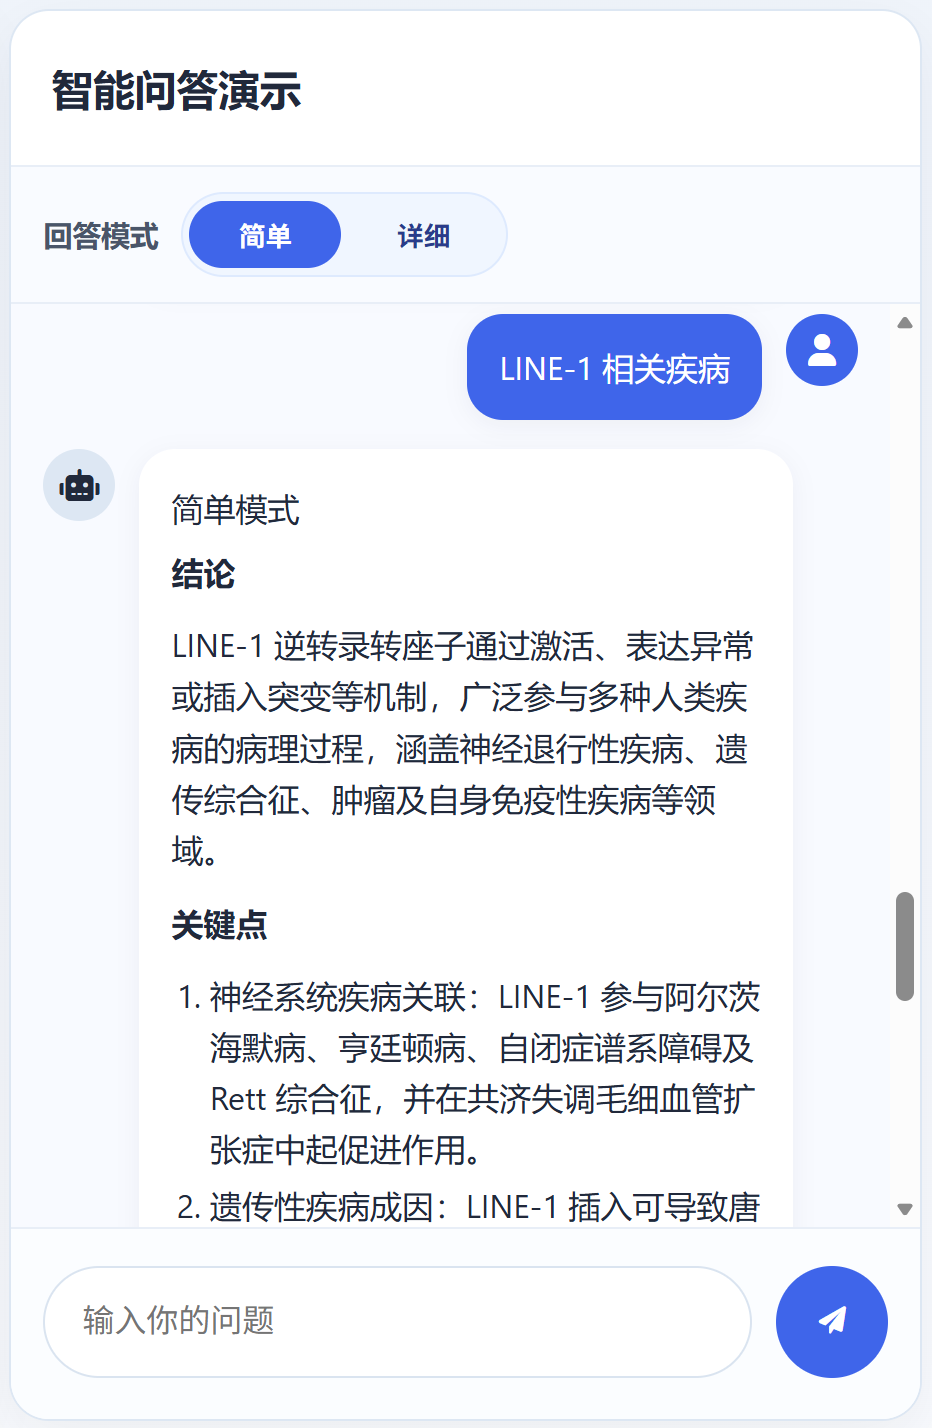
\includegraphics[width=\linewidth]{figures/fig_qa_simple.png}
    \caption{简单模式问答示例}
    \label{fig:qa-simple}
  \end{subfigure}
  \hfill
  \begin{subfigure}[t]{0.48\linewidth}
    \centering
    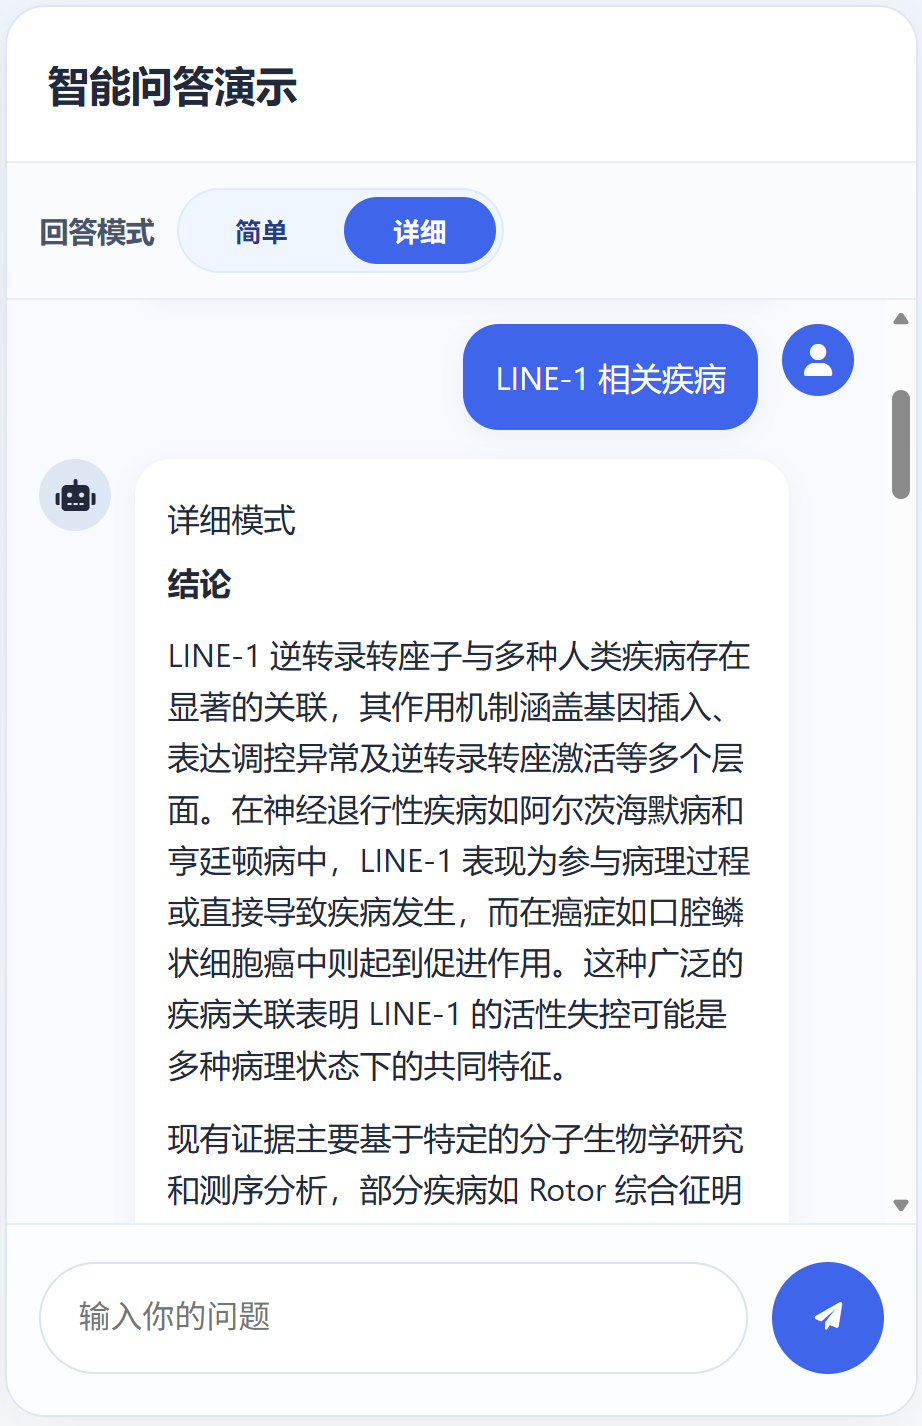
\includegraphics[width=\linewidth]{figures/fig_qa_detailed.png}
    \caption{详细模式问答示例}
    \label{fig:qa-detailed}
  \end{subfigure}
  \caption{智能问答模块的简单模式与详细模式展示}
  \label{fig:qa-mode-pair}
\end{figure}
